\section{Baseline}

\subsection{Overall Architecture}
\begin{figure}[h!]
    \centering
    \includegraphics[width=1\linewidth]{images/mono3dv/baseline_overall.png}
    \caption{The overall framework of MonoDETR.}
    \label{fig:monodetr_baseline}
\end{figure}

The MonoDETR~\cite{MonoDETR} framework presents an end-to-end transformer-based architecture for monocular 3D object detection. Unlike center-based approaches that rely on local pixel-level features, MonoDETR introduces a depth-guided paradigm to capture scene-level geometric cues and long-range object dependencies. As shown in \Cref{fig:monodetr_baseline}, the pipeline consists of a backbone network, a Depth-Guided Transformer, and a set of detection heads.

Given an input image $I \in \mathbb{R}^{H \times W \times 3}$, a backbone network (e.g., ResNet-50) extracts multi-scale feature maps. These features are processed to generate two distinct representations: visual features $F_V$ containing appearance information, and depth features $F_D$ encoding geometric structure. These representations are subsequently fused in the transformer to predict a set of 3D object candidates without the need for Non-Maximum Suppression (NMS).

\subsection{Depth-Guided Transformer}
The core innovation of MonoDETR is the integration of explicit depth supervision into the transformer architecture, enabling the model to learn depth-aware representations.

\noindent\textbf{Depth Predictor and Encoder.}
To mitigate the depth ambiguity inherent in monocular images, a lightweight depth predictor is employed. It takes the backbone features as input and predicts a foreground depth map $D_{pred}$. This predictor is supervised by object-wise discrete depth labels derived from the 3D ground truth, avoiding the need for dense depth annotations.
The predicted depth information is embedded into a high-dimensional feature space to form the depth embeddings $F_D$. Simultaneously, the visual features are flattened and supplemented with positional encodings to form the visual embeddings $F_V$. Both $F_D$ and $F_V$ are refined via separate encoder branches to capture global context.

\noindent\textbf{Depth-Guided Decoder.}
The decoder transforms a set of learnable object queries $Q \in \mathbb{R}^{N \times C}$ into 3D detection predictions. Unlike standard DETR decoders, MonoDETR introduces a \textit{Depth Cross-Attention (DCA)} module to explicitly guide the queries with geometric cues. The decoding process for each layer $l$ proceeds as follows:

1.  \textbf{Depth Cross-Attention:} The object queries attend to the depth embeddings $F_D$ to acquire geometric context.
    \begin{equation}
        Q'_{l} = \text{MHCA}(Q_{l-1}, K=F_D, V=F_D)
    \end{equation}
    where MHCA denotes Multi-Head Cross-Attention. This step ensures that the queries are initialized with scene-level depth information before processing visual appearance.
    
2.  \textbf{Self-Attention:} The queries interact with each other to model inter-object relations.
    \begin{equation}
        Q''_{l} = \text{MHSA}(Q'_{l})
    \end{equation}
    
3.  \textbf{Visual Cross-Attention:} The depth-informed queries then aggregate visual information from $F_V$ using Deformable Attention to focus on relevant image regions efficiently.
    \begin{equation}
        Q_{l} = \text{DeformAttn}(Q''_{l}, P_q, F_V)
    \end{equation}
    where $P_q$ represents the reference points predicted from the queries.

\subsection{Bipartite Matching and Loss}
MonoDETR formulates 3D detection as a set prediction problem. Let $y = \{y_i\}_{i=1}^{M}$ be the ground truth set of objects and $\hat{y} = \{\hat{y}_i\}_{i=1}^{N}$ be the set of $N$ predictions. A bipartite matching between ground truth and predictions is established using the Hungarian algorithm to minimize the matching cost $L_{match}$.

\noindent\textbf{Matching Cost.}
The matching cost considers both classification accuracy and 3D bounding box similarity. For a ground truth $y_i$ and a prediction $\hat{y}_{\sigma(i)}$ with index $\sigma(i)$, the cost is defined as:
\begin{equation}
    \mathcal{L}_{match}(y_i, \hat{y}_{\sigma(i)}) = -\lambda_{cls} \hat{p}_{\sigma(i)}(c_i) + \lambda_{box} \mathcal{L}_{box}(b_i, \hat{b}_{\sigma(i)})
\end{equation}
where $\hat{p}_{\sigma(i)}(c_i)$ is the probability of class $c_i$.

\noindent\textbf{Loss Function.}
The total training loss $L_{total}$ combines the Hungarian loss for the optimal matching $\hat{\sigma}$ and the auxiliary depth loss:
\begin{equation}
    L_{total} = \sum_{i=1}^{M} \left[ L_{cls}(c_i, \hat{c}_{\hat{\sigma}(i)}) + L_{box}(b_i, \hat{b}_{\hat{\sigma}(i)}) \right] + \lambda_{depth} L_{depth}
\end{equation}

\begin{itemize}
    \item \textbf{Classification Loss ($L_{cls}$):} A Focal Loss is utilized to handle class imbalance.
    \item \textbf{3D Bounding Box Loss ($L_{box}$):} This term is a weighted sum of losses for different 3D attributes:
    \begin{equation}
        L_{box} = \lambda_{L1} ||b_i - \hat{b}_{\hat{\sigma}(i)}||_1 + \lambda_{GIoU} L_{GIoU}(b^{2D}_i, \hat{b}^{2D}_{\hat{\sigma}(i)})
    \end{equation}
    where $L_{GIoU}$ is the Generalized IoU loss applied to the projected 2D bounding boxes, and the L1 loss is applied to the regression of 3D center $(x, y, z)$, dimensions $(h, w, l)$, and orientation $\theta$.
    \item \textbf{Depth Loss ($L_{depth}$):} The depth predictor is supervised by a classification loss (e.g., Focal Loss) against the discretized object-wise depth labels, ensuring the depth embeddings $F_D$ carry meaningful geometric information.
\end{itemize}

\subsection{Problem and Motivation}
MonoDETR~\cite{MonoDETR} pioneered a DETR-based framework for monocular 3D detection, using a depth-guided transformer. Although this architecture significantly improved object localization over prior methods, its reliance on a Bipartite Matching setup with only 2D attributes creates an inherently suboptimal optimization. Specifically, as illustrated in \Cref{fig:motivation_3d_matching}, the matching process can prioritize a candidate prediction with a superior 2D bounding box, even if its associated 3D bounding box is inferior. This mismatch causes the better 3D prediction to be incorrectly discarded from the training loss by the 2D-only matching mechanism.


Although MonoDETR~\cite{MonoDETR} initially integrated the 3D attribute into the Bipartite Matching, naively combining the 3D attribute can lead to training collapse, which is caused by instability in 3D prediction in the early training stage. To address these issues, we proposed 3D-Aware Bipartite Matching, which incorporates the 3D attribute into the Bipartite Matching process via a scheduler. Additionally, we introduced 3D DeNoising to mitigate the instability that arises when using the 3D attribute for Bipartite Matching due to the ill-posed nature of 3D estimation from monocular images. Furthermore, we observed the gradient vanishing problem encountered with conventional denoising approaches and presented Variational Query DeNoising to overcome it, which significantly enhances the model's performance.

\begin{figure*}[h!]
    \centering
    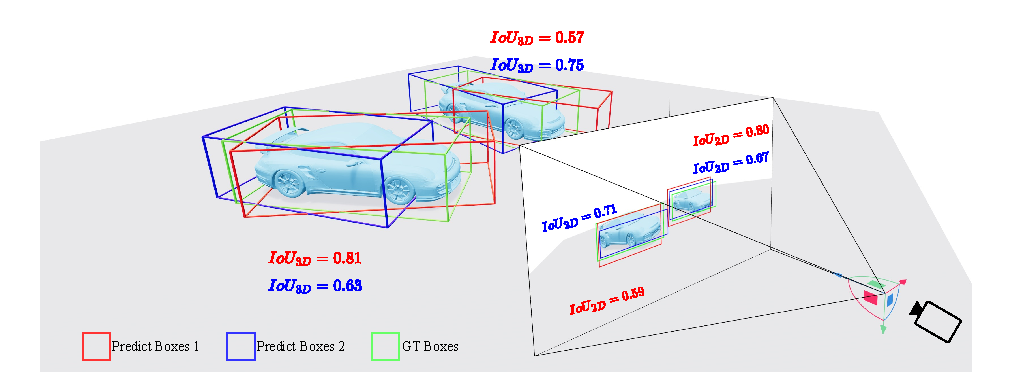
\includegraphics[width=\textwidth]{images/mono3dv/motivation_3d_matching.pdf}
    \caption{\textbf{Limitations of 2D-only Bipartite Matching.} A major limitation of using a 2D-only matching cost for bipartite assignment is that it prioritizes high-quality 2D predictions even if their associated 3D bounding boxes are poor. Conversely, superior 3D predictions are often discarded if their 2D projection is merely sufficient. This leads to suboptimal optimization because the model is trained based on 2D fidelity rather than the desired 3D accuracy.}
    \label{fig:motivation_3d_matching}
\end{figure*}